\documentclass[11pt]{article}
% Packages and macros shared with the proposal.
\usepackage[letterpaper,margin=1in]{geometry}
\usepackage[T1]{fontenc}
\usepackage{mathpazo}
\usepackage{microtype}
\usepackage{amsmath,amssymb,amsthm,stmaryrd}
\usepackage{booktabs,tabularx,array}
\usepackage{graphicx}
\usepackage{xcolor}
\usepackage{tikz}
\usetikzlibrary{positioning,arrows.meta,shapes.geometric,fit}
\usepackage{listings}
\usepackage[font=small,labelfont=bf]{caption}
\usepackage{enumitem}
\usepackage[numbers,sort&compress]{natbib}
\usepackage{xurl}
\usepackage[colorlinks=true,linkcolor=blue!50!black,citecolor=blue!50!black,urlcolor=blue!50!black]{hyperref}

\theoremstyle{plain}
\newtheorem{proposition}{Proposition}
\newtheorem{theorem}{Theorem}
\newtheorem{corollary}{Corollary}
\newtheorem{lemma}{Lemma}
\theoremstyle{definition}
\newtheorem{definition}{Definition}
\newtheorem{remark}{Remark}
\newtheorem*{problem}{Problem Statement}

\newcommand{\sem}[1]{\llbracket #1 \rrbracket}
\newcommand{\Lang}{\mathcal{L}}
\newcommand{\IR}{\mathsf{IR}}
\newcommand{\todo}[1]{\textcolor{red}{[TODO: #1]}}

\lstdefinestyle{q}{basicstyle=\ttfamily\footnotesize,columns=fullflexible,keepspaces=true,breaklines=true}
\lstset{style=q}

% --- build variants -------------------------------------------------------------
% `\iffull` is set by the top-level file: true in main_full.tex, false in main.tex.
% An apparatus file begins with \apphead so that it is a subsection of the section it
% belongs to when inline, and an appendix section when deferred.
\newcommand{\apphead}[2]{\iffull\subsection{#1}\else\section{#1}\fi\label{#2}}
% \inlineonly{...} is prose that only makes sense where the material is in place.
\newcommand{\inlineonly}[1]{\iffull#1\fi}
% \shortonly{...} is the inverse of \inlineonly: a condensation that stands in for
% deferred material in the build that defers it, and would merely restate it in the complete
% one, where the material itself is a paragraph away. Its figures stay in the source
% either way, so tests/test_paper_figures.py still holds it to the registry.
\newcommand{\shortonly}[1]{\iffull\else#1\fi}
% Point at apparatus wherever this build put it, so one sentence reads correctly in both.
% The appendix wrappers are deferred-build-only and so are their labels, so the inline
% build cannot cite a number --- there the material is a few paragraphs down the same
% section. Every call site is therefore written to read with ``below'' as well.
\newcommand{\apref}[1]{\iffull below\else Appendix~\ref{#1}\fi}


\title{\textbf{Switching Costs as a Language-Design Artifact:}\\
\Large Are Observability Query Languages Inter-Translatable?}
\author{Marshall Uy Alexander\\ \small CS 681 Applications of Computability --- Research Paper}
\date{\small \today}

\begin{document}
\maketitle

\begin{abstract}\noindent
\todo{Write last. One sentence each: lock-in problem; thesis; method (grammars, IR,
ingestion mapping, differential testing); headline results (RQ1--RQ3); what it means.}
\end{abstract}

\section{Introduction}
\label{sec:intro}
\todo{Lock-in from proprietary query languages; the migration scenario (Datadog $\to$
Prometheus, going forward); thesis; contributions list: (i) LALR(1) grammars incl.\ first
published Datadog grammar, (ii) $\phi$-relative soundness and the information barrier,
(iii) exact translations of Datadog rollups into PromQL, (iv) gap catalogue, (v) $\kappa$.}

\section{Background and Related Work}
\label{sec:background}
\todo{Condense proposal \S2: Rich \S48.1 and Table of language classes; the languages;
SQL dialect translation (Calcite, SQLGlot); PromQL compliance tester; CNCF query-language
working group; economics of switching costs.}

\section{Formal Framework}
\label{sec:framework}
\todo{Move Definitions 1--4 from the proposal here (data model, query language,
soundness, coverage), with $d$ defined via $|a-b|/\max(|a|,|b|)$.}

% ---------------------------------------------------------------------------
% Ingestion mapping and phi-relative soundness, for the main direction
% (Datadog -> PromQL). Requires \sem, \Lang from macros.tex.
% Numbers come from notebook 02 and data/raw/anchored/ (scripts/verify_anchored.py).
% ---------------------------------------------------------------------------

\subsection{Ingestion and \texorpdfstring{$\phi$}{phi}-relative soundness}
\label{sec:ingestion}

\paragraph{Scope: forward portability.}
The goal is portability of \emph{queries going forward}: once an organization
dual-writes (or switches) its telemetry, a translated query must mean the same thing
as the original on the data each system receives from then on. Migrating stored history
is out of scope. The two systems still do not store the same thing, however, so
soundness must be stated relative to how each ingests data.

\begin{definition}[Ingestion mapping]\label{def:phi}
A Prometheus counter series $s=(\lambda,\langle (t_1,v_1),\dots,(t_n,v_n)\rangle)$ stores
cumulative values. Datadog stores \texttt{COUNT} points that are per-interval deltas. For a
reset policy $\rho\in\{\mathsf{zero},\mathsf{clamp}\}$ define
\[
\phi_\rho(s) = \big(\lambda,\ \langle (t_i,\ \delta_\rho(v_{i-1},v_i)) : 2\le i\le n \rangle\big),
\]
\[
\delta_\rho(u,v)=\begin{cases}
v-u & v\ge u\\
v & v<u,\ \rho=\mathsf{zero}\quad\text{(restarted from $0$, as PromQL assumes)}\\
0 & v<u,\ \rho=\mathsf{clamp}\quad\text{(the decrease contributes nothing)}
\end{cases}
\]
Every series that is not a counter --- a gauge, and the $\mathsf{delta}$ kind
Definition~\ref{def:model} also admits --- maps by the identity, so $\phi_\rho$ is total
on $\mathcal{D}$ and the statements below may quantify over all of it.
$\phi_\rho$ extends to databases series by series:
$\phi_\rho(D)=\{\phi_\rho(s): s\in D\}$. The first sample is omitted. For the agent path
this paper models, that is read from the agent's source rather than from
documentation~\citep{ddagent}, as Remark~\ref{rem:rho} describes; Datadog documents the
same rule for its OTLP path, where a cumulative monotonic sum is differenced and the
first point stored but omitted~\citep{ddotlp}. Every claim below names the
$\rho$ it holds for.
\end{definition}

\begin{remark}[Which $\rho$, and how we know]\label{rem:rho}
Datadog's documentation does not say what becomes of a counter decrease. Its agent is
open source, so the question can be answered by reading it~\citep{ddagent}, and then put
to a running one; both were done and they agree. The reading first.

The conversion carries a per-sample flag. With the flag set, a
sample below its predecessor contributes its own value, on the agent's stated assumption
that the counter restarted from zero --- this is $\delta_{\mathsf{zero}}$ term for term.
With the flag clear, the decrease contributes nothing and the point is still emitted,
which is $\delta_{\mathsf{clamp}}$. The OpenMetrics check sets the flag after every
successful scrape, so the ingestion path this paper models is $\phi_{\mathsf{zero}}$ from
its second scrape onward: the policy PromQL's own reset handling assumes.

Both branches above are thus implemented, and a third that an earlier draft of this
section offered --- discarding the interval outright --- is not, at least not as a reset
policy. Discarding is instead what happens at the \emph{start} of a series, where there is
no predecessor to difference against. A failed scrape is the interesting case: it clears
the flag, so the next interval is converted under $\mathsf{clamp}$ rather than
$\mathsf{zero}$, and is dropped altogether if the aggregator's stored predecessor has
expired in the meantime. Either way a transient failure perturbs $\phi(D)$ in a way
nothing applied to $D$ reproduces, and Proposition~\ref{prop:admissible} gives no warning,
because the discrepancy is between the two stored databases rather than between two
queries. No refusal can flag it and no translation can repair it.

Reading the agent establishes what it intends to send, not what the backend stores, and
the two are different claims. E1 closes the gap by putting a real agent in the loop. A
local endpoint exposes a counter that climbs by one per scrape to $1000$ and then, inside
one rollup bucket, drops to $100$; a Datadog Agent runs an OpenMetrics check against it
and a Prometheus scrapes the same endpoint. Over the bucket holding the reset Datadog
stores $\mathbf{103}$ across four points --- the increment before the reset, the new
value reported as the reset interval's own count, and the two increments after it. That
is $\delta_{\mathsf{zero}}$ and nothing else: $\mathsf{clamp}$ predicts $3$ over four
points, discarding the interval predicts $3$ over three, and a backend keeping the signed
difference predicts $-897$. The four predictions were recorded before the run and are
regression-tested in \texttt{tests\slash test\_reset.py}. A second counter resetting to
exactly $0$ rather than $100$ reads $3$, which is what $\mathsf{zero}$ requires and rules
out a special case at zero; a third that never resets reads four increments of one in
every bucket, which is what shows the run is reading the bucket it means to.
\end{remark}

\begin{remark}[$\phi_\rho$ and the flush interval]\label{rem:flush}
$\phi_\rho$ differences consecutive \emph{samples}, and the agent aggregates samples
into the interval it flushes. An earlier version of this remark inferred from the source
that the two part company as soon as a flush holds more than one sample: a decrease
appeared to \emph{overwrite} what the interval had accumulated rather than adding to it,
so a flush holding an increase and then a reset should report the post-reset value alone,
where $\phi_{\mathsf{zero}}$ keeps both. The agent's default scrape and flush intervals
are both $15$\,s, which would make the question moot in the default configuration and
was the reason it went untested.

Put to a running agent, it does not happen --- though not quite for the reason the run
was designed to test, and the difference is worth keeping. Driving the OpenMetrics
check at a $5$\,s collection interval against the unchanged $15$\,s flush, the bucket
holding the reset reports $111$: eleven increments of one and the reset's own value,
which is $\phi_{\mathsf{zero}}$ term for term. Losing the increment that shares a flush
with the reset would give $110$ (\texttt{scripts\slash reset\_policy.py -{}-step 5}).

What the stored data then shows is that no flush combined anything. Every complete
$60$\,s bucket holds twelve points, one per collection, where three samples to a flush
would have left four. So the agent forwarded each sample rather than aggregating within
the flush, and the overwrite this remark used to posit had no opportunity to occur. The
hypothesis is therefore unexercised rather than refuted, and what the run does
establish is the end-to-end fact the exactness claims actually use: at this ratio
Datadog stores $\phi_{\mathsf{zero}}$ term for term, so those claims do not depend on
the scrape and flush intervals agreeing. The ratio itself was configured and not
observed --- the record computes it from the two interval settings --- and no run here
drives it to a point where a flush must combine samples.
\end{remark}

\paragraph{The dual-write model.}
In the migration this paper is about, one stream of counter observations reaches both
systems. Prometheus stores the cumulative series $D$; Datadog stores $\phi_\rho(D)$. A
Datadog query therefore reads $\phi_\rho(D)$ and its PromQL translation reads $D$. Write
$\sem{\cdot}_{\mathrm{DD}}$ and $\sem{\cdot}_{\mathrm{PQ}}$ for the two denotations.

\begin{definition}[$\phi$-relative $\varepsilon$-soundness]\label{def:phi-sound}
Let $\mathcal{C}\subseteq\mathcal{D}$ be a class of databases. A translation $T$ from
Datadog to PromQL is \emph{$\varepsilon$-sound for $\phi_\rho$ on $\mathcal{C}$ along an
evaluation map $u$} if
\[
\forall q\in \Lang(G_{\mathrm{DD}}).\; T(q)\neq\bot \Rightarrow \forall D\in\mathcal{C},\ t\in\mathbb{T}.\;\;
d\big(\sem{q}_{\mathrm{DD}}(\phi_\rho(D),t),\ \sem{T(q)}_{\mathrm{PQ}}(D,u(t))\big)\le\varepsilon .
\]
The evaluation map is not bookkeeping. Remark~\ref{rem:closure} measures Datadog's
buckets as left-closed and labelled by their start, and a PromQL range window as
right-closed; no single instant reads both, so a definition quantifying one $t$ over both
sides has no positive instance in this paper. Every exactness result below names its
$u$, and each is $u(t)=t+\Delta-\eta$.
Definition~\ref{def:sound} is the special case
$\phi_\rho=\mathrm{id}$.
\end{definition}

\begin{definition}[$\phi$-invariance]\label{def:phi-inv}
A PromQL expression $p$ is \emph{$\phi_\rho$-invariant on $\mathcal{C}$} if for all
$D,D'\in\mathcal{C}$ and all $t$:
$\phi_\rho(D)=\phi_\rho(D')\Rightarrow \sem{p}_{\mathrm{PQ}}(D,t)=\sem{p}_{\mathrm{PQ}}(D',t)$;
that is, $\sem{p}_{\mathrm{PQ}}$ factors through $\phi_\rho$.
\end{definition}

\noindent
Invariance is what makes an expression \emph{usable as a translation} here. The source
query cannot distinguish two databases with the same $\phi_\rho$ image, so a sound
translation must not distinguish them either.

\begin{proposition}[Admissibility]\label{prop:admissible}
Let $q$ be a Datadog query and $p=T(q)\neq\bot$. If $p$ is not $\phi_\rho$-invariant on
$\mathcal{C}$, witnessed by $D,D'\in\mathcal{C}$ and $t$, then $T$ is not
$\varepsilon$-sound for $\phi_\rho$ on $\mathcal{C}$ for any
$\varepsilon<\tfrac12\,d\big(\sem{p}_{\mathrm{PQ}}(D,t),\sem{p}_{\mathrm{PQ}}(D',t)\big)$.
\end{proposition}
\begin{proof}
Since $\phi_\rho(D)=\phi_\rho(D')$, the source query receives the same input in both
cases:
\[
r:=\sem{q}_{\mathrm{DD}}(\phi_\rho(D),t)=\sem{q}_{\mathrm{DD}}(\phi_\rho(D'),t).
\]
Soundness would give $d(r,\sem{p}_{\mathrm{PQ}}(D,t))\le\varepsilon$ and
$d(r,\sem{p}_{\mathrm{PQ}}(D',t))\le\varepsilon$. Because $d$ is a metric on results with
matching label sets (and $\infty$ otherwise), the triangle inequality yields
\[
d\big(\sem{p}_{\mathrm{PQ}}(D,t),\sem{p}_{\mathrm{PQ}}(D',t)\big)\le 2\varepsilon . \qedhere
\]
\end{proof}

\begin{remark}[The barrier is directional]\label{rem:directional}
The same inequality reads differently in the two directions, and the difference is the
reason this paper takes Datadog $\to$ PromQL as the main one.

In the \emph{reverse} direction the source is PromQL, reading $D$, and the target is
Datadog, reading $\phi_\rho(D)$. The constraint then falls on the \emph{source}: a PromQL
query that is not $\phi_\rho$-invariant has no sound Datadog translation at all, for any
target query whatsoever, because every candidate receives the same input on two
databases the source query separates. That is an information barrier in the strict
sense, and it is independent of syntax: such a query is untranslatable because of what
the target system stores, not because of how its language is written. This is the formal
sense in which part of the lock-in is semantic.

In the \emph{main} direction no source query is blocked this way. Prometheus stores $D$
and Datadog's view $\phi_\rho(D)$ is a function of it, so the target system never holds
less than the source did. What Proposition~\ref{prop:admissible} constrains instead is
the \emph{choice of target expression}: a PromQL expression that reads absolute counter
values cannot translate any Datadog query, because no Datadog query can see them.
Sufficient information, however, is not the same as sufficient expressiveness --- to
reproduce $\sem{q}_{\mathrm{DD}}(\phi_\rho(D),t)$ from $D$, PromQL must be able to
\emph{say} the composite $\sem{q}_{\mathrm{DD}}\circ\phi_\rho$.

That holds for the metric types $\phi_\rho$ is defined on, which are the counters and
gauges of Definition~\ref{def:phi}, and it fails for a third.
Corollary~\ref{cor:quantile} exhibits a Datadog query that is blocked informationally in
the main direction, so the barrier is directional for the ingestion path this paper
models rather than for Datadog as a whole --- a distinction an earlier draft of this
remark elided by saying that no refusal in this direction is an informational one. Section~\ref{sec:gaps} keeps the three apart --- what Prometheus does
not hold, what PromQL cannot say, and what this translator has not built --- and the
first two together account for $1.2\%$ of the corpus against the third's $2.4\%$.
\end{remark}

\begin{corollary}[Raw selectors are inadmissible]\label{cor:raw}
Let $\mathcal{C}_{\mathrm{flat}}$ be the databases with no counter reset. On
$\mathcal{C}_{\mathrm{flat}}$, shifting every sample of a series by a constant $c$ leaves
$\phi_\rho$ unchanged while changing the value of a raw selector. Hence a bare counter
selector (\texttt{http\_requests\_total} with no range function), and any function of
absolute counter values, is not $\phi_\rho$-invariant, and no such expression is a sound
translation of any Datadog query. The translator cannot emit one, and by construction
rather than by a runtime check: lowering wraps every selector in a rollup before the
emitter sees it, so no input reaches a bare counter selector. The code
\texttt{PHI\_ABSOLUTE} is reserved for the reverse direction, where the same corollary
does bite.
\end{corollary}

\begin{proposition}[A quantile is not a function of a bucketing]\label{prop:quantile}
Let $B$ be any finite set of bucket boundaries and $0<p<1$. There are finite multisets
$X,Y$ of observations with identical $B$-bucket counts and $q_p(X)\neq q_p(Y)$.
\end{proposition}
\begin{proof}
Let $[a,c)$ be a bucket of $B$ of positive width, which exists whenever $|B|\ge2$; for
$|B|\le1$ take the unbounded bucket and any two distinct positive observations. Put
$m=(a+c)/2$ and let $X=\{m-r,\,m+r\}$ for any $0<r<(c-a)/2$, and $Y=\{m,m\}$. Both put
$2$ in $[a,c)$ and nothing elsewhere, so their bucket counts agree; and both have sum
$2m$ and count $2$. Their medians are $m-r$ and $m$ under any convention that returns an
observed value, so $q_p$ differs.

The witness is chosen to survive more than the bucket counts, which is what the
corollary below needs and what an earlier version of this proof did not supply. It took
$X$ to be $n$ copies of $a$ against $n$ copies of $(a+c)/2$: those agree on bucket counts
and differ in their \emph{sum}, so \texttt{histogram\_sum} separates them and they
witness nothing about expressions over everything Prometheus stores.
\end{proof}

\begin{corollary}[Datadog's percentile aggregators are blocked by information]%
\label{cor:quantile}
A Datadog distribution metric answers $\mathtt{p}NN$ from a sketch of the raw
observations. What Prometheus stores of those observations is a bucketing together with
their sum and their count --- \texttt{\_bucket}, \texttt{\_sum} and \texttt{\_count}
series classically, an exponential bucketing with a Sum and a Count under native
histograms --- and Proposition~\ref{prop:quantile}'s witness agrees on all three while
its quantiles differ. So no PromQL expression over what Prometheus holds equals
$\mathtt{p}NN$, for any expression whatsoever, and the refusal is informational rather
than a shortage of operators: PromQL has \texttt{histogram\_quantile}, and what it
computes is an interpolation within a bucket rather than the quantile itself.

Naming the sum and the count explicitly is the eighth review pass's correction. The
corollary used to infer from ``the quantile is not determined by the bucket counts'', and
Prometheus holds more than the bucket counts --- so the step did not reach the quantifier
the sentence claims, even though the conclusion is true.
\end{corollary}

\noindent
Two things about Corollary~\ref{cor:quantile} are worth keeping separate. It is not a
claim that Datadog is more precise --- a sketch is a lossy summary too, with its own
relative-error bound --- but that the two systems keep \emph{different} lossy summaries
of one stream, and neither is recoverable from the other. And it is the reason the
$34$ percentile occurrences of \S\ref{sec:gaps} carry \texttt{PHI\_QUANTILE} rather
than \texttt{UNSUPPORTED\_FUNCTION}: an earlier draft filed them under a missing
operator, which named the wrong obstruction and put them in the same row as work that
had simply not been done.

\begin{corollary}[\texttt{rate} is inadmissible in general]\label{cor:rate}
PromQL \texttt{rate} is not $\phi_\rho$-invariant on $\mathcal{D}$. When a series begins
inside the window, Prometheus limits start-of-window extrapolation using the absolute
first sample value $v_1$ --- the documentation says only that the calculation
extrapolates to the ends of the range~\citep{promql}; the dependence on $v_1$ is in the
implementation, where the quantity is named \texttt{durationToZero} --- and $v_1$ is erased by
$\phi_\rho$. It
\emph{is} $\phi_\rho$-invariant on the class $\mathcal{C}_{\mathrm{warm}}$ of databases
in which no counter series begins within a window being evaluated.
\end{corollary}

\noindent
That positive half is weaker than an earlier version of this corollary claimed, and the
reason is worth recording because it is a fact about Prometheus rather than about
$\phi$. The claim was that on $\mathcal{C}_{\mathrm{warm}}$ ``the remaining inputs to the
extrapolation --- the increase over the window and the sample spacing --- all survive
$\phi_\rho$''. They do not exhaust the inputs: when the computed increase is positive,
\texttt{rate} derives a \texttt{durationToZero} from the \emph{absolute value} of the
first sample inside the window, and $\phi_\rho$ erases absolute values exactly as it
erases $v_1$. Two databases differing by a constant offset therefore have equal
$\phi_\rho$ images and different \texttt{rate} readings --- $0.628$ against $0.667$ on an
ordinary counter --- and the dependence is confirmed against a real Prometheus~3.15.0
rather than against this paper's model of it. So \texttt{rate} is inadmissible on
$\mathcal{C}_{\mathrm{warm}}$ too, and the class on which it is admissible is smaller
than the one named here. Nothing downstream rests on it: §\ref{sec:translation} cites
Corollary~\ref{cor:raw}, not this one, and \texttt{rate} is never emitted.

\noindent
Corollary~\ref{cor:rate} is worth stating carefully, because it marks the limit of what
invariance buys. Invariance is \emph{necessary} for a sound translation and not
sufficient, and \texttt{rate} fails both: it is inadmissible wherever the extrapolation
reads an absolute value, and even where it is admissible it is not exact, since
extrapolating to the window edges computes a different quantity from the bucket sum
Datadog reports. Admissibility rules candidates out; exactness has to be established
separately.

\subsubsection{Two exact forms}

Datadog's \texttt{.as\_count()} with rollup interval $\Delta$ reports, for the bucket it
labels $b$,
\[
\Sigma_\Delta(b)=\sum\{\,\delta : (t_i,\delta)\in\phi_\rho(s),\ t_i\in[b,\,b+\Delta)\,\},
\]
undefined where that set is empty rather than $0$: Datadog reports no point for a bucket
holding no data, and a range selector over the same window returns nothing, so reading
the empty sum as zero would make the two sides disagree exactly where they agree.
\texttt{datadog\_eval} has always reported it as absent; the definition now says so.
and \texttt{.as\_rate()} reports $\Sigma_\Delta(b)/\Delta$. Both reduce to the same
cumulative difference, which is the single most useful fact in this direction: the
corpus of Section~\ref{sec:evaluation} uses \texttt{.as\_count()} about $6.6$ times as
often as \texttt{.as\_rate()}.

\begin{remark}[Which interval a bucket covers, measured]\label{rem:closure}
That the bucket is \emph{left}-closed and named by its \emph{start} is measured rather
than assumed, and it is not what we first assumed. Submitting one point at an exact
multiple of $\Delta$ and one strictly inside a bucket, and reading back which bucket each
is reported under, separates the four conventions: a point on a boundary is reported
under the bucket \emph{starting} there. Each of the other three conventions is ruled out
by at least one of the two readings (\texttt{scripts\slash trial\_checks.py e2}; the
responses are cached and regression-tested). It is one run at one rollup interval ---
the script fixes $\Delta$ at $60$\,s --- so what is pinned is the convention at that
width, not its independence of the width.

The convention PromQL uses for its own range selectors is the opposite one, $(u-w,u]$,
which is why it was the natural guess. Getting it wrong cost nothing numerically --- a
model and a candidate evaluated under the same convention agree with each other, so every
figure in Table~\ref{tab:rollup-live} is what it was --- but it was a claim about Datadog
that happened not to be true, and it changes where a translated query must be evaluated.
\end{remark}

\noindent
It changes it in a way that is easy to get wrong twice. Since a PromQL range selector
covers $(u-\Delta,u]$ and the bucket covers $[b,b+\Delta)$, no instant makes the two
cover the same samples when a sample lands on a boundary: at $u=b+\Delta$ the window
takes the sample at $b+\Delta$, which Datadog has put in the next bucket, and misses the
one at $b$, which Datadog has put in this one. With a scrape interval that divides the
rollup interval --- the ordinary case --- that is every bucket. The evaluation instant
must therefore lie strictly \emph{inside} the bucket.

\begin{proposition}[Cumulative difference]\label{prop:offset}
Let $\mathcal{C}_{\Delta}$ be the databases in which no counter series resets within
$[b,b+\Delta)$ \emph{and every counter series has a sample before $b$}. For such a
database write $t_m$ for the last sample in $[b,b+\Delta)$ and $t_k$ for the last sample
before $b$, and let $\eta$ satisfy
\[
0<\eta\le\min\big(b+\Delta-t_m,\ b-t_k\big).
\]
Assume Prometheus's lookback covers both $u-t_m$ and $(u-\Delta)-t_k$ for
$u=b+\Delta-\eta$. Then on $\mathcal{C}_{\Delta}$ the expression
\texttt{x - x offset $\Delta$}, evaluated at $u$, is $\phi_\rho$-invariant and equals
$\Sigma_\Delta(b)$ exactly.
\end{proposition}
\begin{proof}
An instant selector at $u$ returns $v_{\ell(u)}$ for $\ell(u)=\max\{i:t_i\le u\}$,
provided the lookback reaches $t_{\ell(u)}$; the hypothesis grants that at both $u$ and
$u-\Delta$. Since $\eta\le b+\Delta-t_m$ we have $t_m\le u<b+\Delta$, and the next sample
is at or after $b+\Delta>u$, so $\ell(u)=m$; since $\eta\le b-t_k$ we have
$t_k\le u-\Delta<b$, so $\ell(u-\Delta)=k$. With no reset in the bucket,
$\delta_\rho(v_{i-1},v_i)=v_i-v_{i-1}$ for every $t_i\in[b,b+\Delta)$, so the sum
telescopes: $\Sigma_\Delta(b)=v_m-v_k$, which is the value of the expression. It is
$\phi_\rho$-invariant on $\mathcal{C}_\Delta$ because it has been shown equal to a
function of $\phi_\rho(s)$ alone.
\end{proof}

\begin{remark}[Why the bound is not the scrape interval]\label{rem:eta}
An earlier version of this proposition set $0<\varepsilon\le\sigma$ for $\sigma$ the
least gap between consecutive samples, and argued that the next sample after $t_m$ is at
least $\sigma$ beyond it and at or after $b+\Delta$, hence $t_m\le b+\Delta-\sigma$. That
does not follow: the next sample may exceed $b+\Delta$ by any amount, which bounds
nothing. The inference holds only when the sample grid's phase divides $\Delta$, and the
replay of \S\ref{sec:replay} reports the jittered grid as the ordinary deployment case.
On a series scraped every $15$\,s whose last sample inside the bucket sits $14$\,s
before its right edge, the least gap is $15$ while $b+\Delta-t_m$ is $14$, so $\eta=15$
is admitted by the old bound and excluded by the correct one ---
and at $\eta=15$ both exact forms miss the bucket's largest delta entirely, returning a
$d$ close to $1$ where the correct bound returns $0$.
No measurement in this paper is affected, because every script evaluates at
$\eta=10^{-3}$ (\texttt{datadog\_eval.EVAL\_EPSILON}), well inside
$\min(b+\Delta-t_m,\,b-t_k)$ on every grid it uses; the implementation's own docstring
states the correct condition, and the proposition had not caught up with it. The offset
$\eta$ is also renamed here: it was written $\varepsilon$, which is Definition~\ref{def:sound}'s
tolerance, and the two appeared in one sentence of Theorem~\ref{thm:kernel}.
\end{remark}

\begin{proposition}[Anchored increase]\label{prop:anchored}
Let $\rho=\mathsf{zero}$, let $t_m,t_k,\eta,u$ be as in
Proposition~\ref{prop:offset}, and assume Prometheus's lookback covers $u-t_a$ for $t_a$
the last sample at or before $u-\Delta$. Then
\texttt{increase(x[$\Delta$] anchored)} evaluated at $u$ equals
$\Sigma_{\mathsf{zero},\Delta}(b)$ whenever the bucket contains a sample, including on
series the second hypothesis of $\mathcal{C}_\Delta$ excludes, and is
$\phi_{\mathsf{zero}}$-invariant.
\end{proposition}
\begin{proof}
The \texttt{anchored} modifier pins the left window boundary to the last
sample at or before $u-\Delta$ and performs no extrapolation, both of which the
proposal states~\citep{prom0052}. What the proposal does not say, and what an earlier
version of this proposition therefore missed, is that the anchor is itself subject to the
lookback: read off a real Prometheus~3.15.0, a series whose only samples are one at
time zero and three more arriving after a gap of over ten minutes returns $2$ for this
expression over the bucket holding those three, where Datadog returns $12$ --- and
returns $12$ once the server is started with a lookback wide enough to see the first
sample. Hence the hypothesis above, and hence the withdrawal of the claim that
this form is exact on \emph{all} of $\mathcal{D}$: a scrape outage wider than the
lookback defeats it, at any server configuration, which is not the misconfiguration an
earlier draft of Theorem~\ref{thm:kernel} called it. On a decrease $v_i<v_{i-1}$ it contributes $v_i$
rather than $v_i-v_{i-1}$; the proposal says only that the modifier ``deals with
counter resets'', so that clause is taken from the readings of
Table~\ref{tab:model-verification} and Remark~\ref{rem:rho} rather than from the text. Term by term this is exactly
$\delta_{\mathsf{zero}}$, and by the index argument of
Proposition~\ref{prop:offset} the terms it sums are those with
$t_i\in[b,b+\Delta)$, so the total is $\Sigma_{\mathsf{zero},\Delta}(b)$, a function of
$\phi_{\mathsf{zero}}(s)$ alone. The hypothesis that the bucket contains a sample is
needed for the same reason Definition~\ref{def:d}'s first case is: with no sample in
$[b,b+\Delta)$ the range selector returns nothing while $\Sigma_\Delta(b)$ is an empty
sum, and a number is not an absent result. \texttt{datadog\_eval} reports the empty
bucket as absent on both sides, which is what Datadog does and what this proposition now
says.
\end{proof}

\begin{remark}[The second hypothesis, and the second advantage]\label{rem:series-start}
The series-start hypothesis was missing from an earlier statement of
Proposition~\ref{prop:offset}, whose proof names ``the last sample before $b$'' without
requiring one to exist. When none does, \texttt{x offset $\Delta$} selects nothing and
the difference returns \emph{no result} where Datadog returns the sum of the deltas it
holds --- a disagreement that $d$ scores as $\infty$ rather than as a large number,
since the two results have different domains. Read off a real server on a bucket holding
two series, one beginning before it and one inside it: the difference returns $25$ for
the first and nothing for the second, where $\phi_{\mathsf{zero}}$ sums the second's
deltas to $20$.

The same reading gives the anchored form more than Proposition~\ref{prop:anchored} was
stated to claim. \texttt{increase(x[$\Delta$] anchored)} returns $25$ and $20$ --- both
of Datadog's figures, the new series included. So the anchored form's advantage over the
cumulative difference is not only that it survives a reset; it is also the only one of
the two that is right about a series younger than the window. For a migration that is
the more common case of the two, since every series is new on the day the dual-write
starts, and it is the reason the emitter now records \texttt{PHI\_SERIES\_START}
alongside \texttt{COUNTER\_RESET} on the plain form. The mean-of-deltas rule of
\S\ref{sec:emission} carries it for a second reason: its denominator counts samples
where Datadog counts deltas, and a series beginning inside the bucket has one fewer
delta than it has samples.
\end{remark}

\noindent
Propositions~\ref{prop:offset} and~\ref{prop:anchored} explain the measurements rather
than merely accompanying them. The cumulative difference is exact exactly where its
invariance class holds --- no reset inside the window --- and the anchored form, whose
reset handling \emph{is} $\delta_{\mathsf{zero}}$, is exact everywhere. Both are
confirmed in Table~\ref{tab:rollup-live}: over four synthetic workloads at two rollup
intervals, the cumulative difference agrees with the modelled rollup on every bucket of
the reset-free workloads and falls to between $91.4\%$ and $98.3\%$ once counters
restart, with relative
error as large as $1.68$, while the anchored form is exact on every bucket of every
workload. ``Modelled'' is the right word there and is not a hedge: that table reads
Datadog's side from the reference evaluator of \S\ref{sec:replay}, and it is the replay
of \S\ref{sec:replay} and the scripted reset of Remark~\ref{rem:rho} that put the same
claims to the system itself. \texttt{rate} is exact only on perfectly regular traffic.

\begin{table}[htbp]\centering\footnotesize
\begin{tabular}{@{}lrlrrr@{}}
\toprule
Workload & $\Delta$ (s) & PromQL candidate & Exact & Median $d$ & Max $d$ \\
\midrule
bursty & 300 & \texttt{rate(x[$\Delta$])} & 0\% & 0.017 & 0.065 \\
bursty & 300 & \texttt{(x - x offset $\Delta$) / $\Delta$} & 100\% & 0.000 & 0.000 \\
bursty & 300 & \texttt{increase(x[$\Delta$] anchored) / $\Delta$} & 100\% & 0.000 & 0.000 \\
bursty & 60 & \texttt{rate(x[$\Delta$])} & 0\% & 0.137 & 0.750 \\
bursty & 60 & \texttt{(x - x offset $\Delta$) / $\Delta$} & 100\% & 0.000 & 0.000 \\
bursty & 60 & \texttt{increase(x[$\Delta$] anchored) / $\Delta$} & 100\% & 0.000 & 0.000 \\
bursty + restarts & 300 & \texttt{rate(x[$\Delta$])} & 0\% & 0.017 & 0.065 \\
bursty + restarts & 300 & \texttt{(x - x offset $\Delta$) / $\Delta$} & 92\% & 0.000 & 1.679 \\
bursty + restarts & 300 & \texttt{increase(x[$\Delta$] anchored) / $\Delta$} & 100\% & 0.000 & 0.000 \\
bursty + restarts & 60 & \texttt{rate(x[$\Delta$])} & 0\% & 0.137 & 0.750 \\
bursty + restarts & 60 & \texttt{(x - x offset $\Delta$) / $\Delta$} & 98\% & 0.000 & 1.156 \\
bursty + restarts & 60 & \texttt{increase(x[$\Delta$] anchored) / $\Delta$} & 100\% & 0.000 & 0.000 \\
poisson & 300 & \texttt{rate(x[$\Delta$])} & 0\% & 0.013 & 0.056 \\
poisson & 300 & \texttt{(x - x offset $\Delta$) / $\Delta$} & 100\% & 0.000 & 0.000 \\
poisson & 300 & \texttt{increase(x[$\Delta$] anchored) / $\Delta$} & 100\% & 0.000 & 0.000 \\
poisson & 60 & \texttt{rate(x[$\Delta$])} & 0\% & 0.142 & 0.322 \\
poisson & 60 & \texttt{(x - x offset $\Delta$) / $\Delta$} & 100\% & 0.000 & 0.000 \\
poisson & 60 & \texttt{increase(x[$\Delta$] anchored) / $\Delta$} & 100\% & 0.000 & 0.000 \\
steady & 300 & \texttt{rate(x[$\Delta$])} & 100\% & 0.000 & 0.000 \\
steady & 300 & \texttt{(x - x offset $\Delta$) / $\Delta$} & 100\% & 0.000 & 0.000 \\
steady & 300 & \texttt{increase(x[$\Delta$] anchored) / $\Delta$} & 100\% & 0.000 & 0.000 \\
steady & 60 & \texttt{rate(x[$\Delta$])} & 100\% & 0.000 & 0.000 \\
steady & 60 & \texttt{(x - x offset $\Delta$) / $\Delta$} & 100\% & 0.000 & 0.000 \\
steady & 60 & \texttt{increase(x[$\Delta$] anchored) / $\Delta$} & 100\% & 0.000 & 0.000 \\
\bottomrule
\end{tabular}

\caption{Agreement of three PromQL candidates with Datadog's \texttt{.as\_rate()} rollup,
read from a Prometheus~3.15.0 server rather than from a model of PromQL. ``Exact'' is the
share of epoch-aligned buckets with $d=0$. Workloads are six hours of $15$\,s scrapes;
``restarts'' zeroes the counter once an hour.}
\label{tab:rollup-live}
\end{table}

\paragraph{Verifying the instruments.}
Propositions~\ref{prop:offset} and~\ref{prop:anchored} are claims about PromQL, so
checking them against our own evaluator would be circular. Each workload is therefore
backfilled into a real Prometheus TSDB, and every candidate is read back from that server
on the same epoch-aligned grid. Table~\ref{tab:model-verification} compares the two: across
$1{,}680$ buckets the reference evaluators and the server agree to floating-point
precision, and there is no bucket where one produced a value and the other declined ---
an empty result is as much a semantic claim as a number. The modelled and measured
versions of Table~\ref{tab:rollup-live} agree on every summary statistic, which the
notebook now asserts cell for cell rather than inviting the reader to compare two
printouts. It did not hold when it was only a sentence: the modelled table took the
warm-up as its first bucket's \emph{start} and the live grid took it as the first
evaluation \emph{instant}, so the two summarised bucket sets one bucket apart --- for
$\Delta=300$ a bucket wholly inside the warm-up --- and six of the twenty-four rows
differed in a printed cell.

\begin{table}[htbp]\centering\footnotesize
\begin{tabular}{@{}lrrr@{}}
\toprule
PromQL candidate & Buckets & Max $d$ vs. server & NaN mismatch \\
\midrule
\texttt{rate(x[$\Delta$])} & 1,688 & 8.60e-14 & 0 \\
\texttt{(x - x offset $\Delta$) / $\Delta$} & 1,688 & 0.00e+00 & 0 \\
\texttt{increase(x[$\Delta$] anchored) / $\Delta$} & 1,688 & 7.95e-16 & 0 \\
\bottomrule
\end{tabular}

\caption{The reference evaluators of \texttt{semantics/promql\_eval.py} against
Prometheus~3.15.0 on identical samples. ``NaN mismatch'' counts buckets where exactly one
of the two returned a value.}
\label{tab:model-verification}
\end{table}

\begin{remark}[\texttt{anchored} is still experimental]\label{rem:anchored-flag}
The \texttt{anchored} modifier of~\citet{prom0052} arrived in Prometheus~3.7.0 behind
\texttt{-{}-enable-feature=promql-extended-range-selectors}, and an earlier draft of this
section asserted that the flag had since become a no-op. It has not. A $3.15.0$ server
started without it rejects the expression outright:
\begin{center}\footnotesize
\texttt{anchored modifier is experimental and not enabled}
\end{center}
The precondition \texttt{ANCHORED\_VERSION} records is therefore stronger than a version
number. It is a server deliberately started with an experimental feature enabled, which
is a different and larger ask of whoever operates the target: a version can be waited
for, a flag has to be chosen. That is the real cost of
Proposition~\ref{prop:anchored}'s exactness, and it is the reason the emitter leaves the
reset-aware form off by default and emits the cumulative difference, which uses nothing
outside standard PromQL.

The error above is how we found out. Every measurement in this paper had been taken with
the flag set, because the script that takes them passes it and a comment there described
it as harmless; the claim was never exercised until a later experiment started a server
without it. A precondition that every instrument satisfies by habit is one nobody tests.
\end{remark}

\begin{remark}[Soundness over all databases is too strong for \texttt{rate}]
Even on $\mathcal{C}_{\mathrm{warm}}$, \texttt{rate} is not $\varepsilon$-sound over all
databases for any $\varepsilon<1$ under relative error: if the whole increase falls
between the last sample before the window and the first sample inside it, one system
returns $0$ while the other counts the delta. Useful bounds must therefore restrict the
data class, e.g.\ to counters whose per-scrape increments vary by at most a factor
$\beta$, and state $\varepsilon$ as a function of $\beta$, the scrape interval $s$ and
the window $w$. Figure~\ref{fig:rate-error} shows how the error shrinks as $\Delta$ grows
relative to the scrape interval.
\end{remark}

\begin{figure}[htbp]\centering
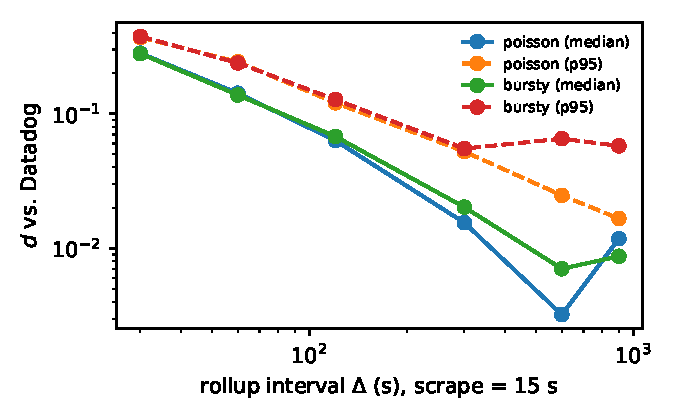
\includegraphics[width=0.6\linewidth]{figures/rate_error_vs_window}
\caption{Error of \texttt{rate()} against Datadog as the rollup interval grows, at a
$15$\,s scrape interval. \texttt{rate} is the only candidate whose error depends on the
data.}
\label{fig:rate-error}
\end{figure}

\subsubsection{The dual-write replay}
\label{sec:replay}

Everything to this point compares a PromQL candidate against our reading of Datadog's
rollup. That is a model, and a model is what \S\ref{sec:not-measured} warns the reader
about. This subsection closes the gap for the counter rules by running the dual-write
construction of this section literally: one stream of observations, written to both
systems, read back from both.

The stream is real. Counting the requests in a web-server access log into a scrape grid
gives a counter with the shape that \S\ref{sec:threats} says the synthetic workloads only
imitate: in the half hour used here the per-minute rate swings seventeenfold without
being asked to. We take the busiest half hour of the Kennedy Space Center HTTP logs of
July~1995~\citep{nasahttp}, count requests at a $15$\,s scrape interval into one counter
per HTTP status class, and write the cumulative series to Prometheus and its image under
$\phi_{\mathsf{zero}}$ --- the per-interval deltas --- to Datadog, at the same timestamps
(\texttt{scripts\slash replay\_dualwrite.py}).
The trace's publishers ask that it not be analysed beyond general traffic patterns, and
the parser enforces that rather than promising it: it keeps a timestamp and a status
class and discards the host and the request line, so what is replayed is a count of
requests per interval and nothing else. Timestamps are shifted to the present, because
Datadog's intake refuses points much older than an hour; the shape is real and the
absolute times are not.

\begin{table}[htbp]\centering\footnotesize
\begin{tabular}{@{}llrrr@{}}
\toprule
Scrape grid & PromQL candidate & Evaluated inside & On the edge & Max $d$ \\
\midrule
unaligned & \texttt{x - x offset $\Delta$} & 100.0\% & 100.0\% & 0 \\
 & \texttt{increase(x[$\Delta$] anchored)} & 100.0\% & 100.0\% & 0 \\
 & \texttt{rate(x[$\Delta$])} $\times\,\Delta$ & 20.2\% & 20.2\% & 1 \\
\addlinespace
aligned & \texttt{x - x offset $\Delta$} & 100.0\% & 27.4\% & 0 \\
 & \texttt{increase(x[$\Delta$] anchored)} & 100.0\% & 27.4\% & 0 \\
 & \texttt{rate(x[$\Delta$])} $\times\,\Delta$ & 20.2\% & 16.7\% & 1 \\
\addlinespace
\bottomrule
\end{tabular}

\caption{The dual-write replay: each candidate against \emph{Datadog}, bucket by bucket,
on a real request trace. ``Inside'' and ``on the edge'' are the two evaluation instants
of Remark~\ref{rem:closure}. $84$ comparisons per row.}
\label{tab:replay}
\end{table}

Table~\ref{tab:replay} is the result, and two things in it are worth separating.

The first is that both exact forms are exact --- against Datadog, not against a model of
it, on traffic nobody generated for the purpose. \texttt{rate} is not, at $20.2\%$ of
buckets on both grids, which is what \S\ref{sec:ingestion} has said throughout and what
the steady synthetic workload conceals by being steady. That figure used to read
$19$--$20\%$, a spread between the two grids that was not a property of either: the
replay script scored this one table by bit-identity where every other exactness column in
this paper uses a $10^{-12}$ relative bound, and one aligned bucket reading $236.0$
against $235.999\ldots$ counted as a disagreement.

The second is about the convention of Remark~\ref{rem:closure}, and it explains how that
convention came to be assumed wrongly for so long. On the unaligned grid --- a scrape
whose samples do not fall on rollup boundaries, which is what a jittered scrape produces
and therefore the ordinary case --- evaluating on the bucket's edge agrees with
evaluating inside it, on every bucket. Off a boundary the two half-open intervals contain
the same samples, so the closure is simply not observable. Snap the scrape grid onto the
rollup grid and the same comparison falls from $100\%$ to $27.4\%$. The error was
invisible in exactly the configuration real deployments have, and decisive in the one the
synthetic workloads of Table~\ref{tab:rollup-live} happen to use.

What this does not do is also worth stating. A request counter does not reset in half an
hour, so \texttt{COUNTER\_RESET} is not exercised here; the restart rows of
Table~\ref{tab:rollup-live} and the scripted reset of E1 (Remark~\ref{rem:rho}) are the
evidence for that case. It is one window of one
trace at one rollup interval. And it tests the counter rules, not translation coverage:
$\kappa$ is what it was.

\paragraph{What was assumed, and what is left.}
This section began with two facts about Datadog that its documentation does not settle,
and carried a third about its backend. None is still an assumption, and the two it began
with did not turn out the way they were guessed.

The reset policy $\rho$ is no longer among them either, and it is the one that was
settled twice: read from the agent's source and then put to a running agent, which
agreed with the reading (Remark~\ref{rem:rho}). It too went against the guess --- the
prediction recorded in advance was discarding the interval, which turns out not to be a
reset policy at all.

Bucket closure is no longer among them. Remark~\ref{rem:closure} settles it by
measurement: buckets are left-closed and named by their start, which is the opposite of
what an earlier draft of this section assumed and the opposite of PromQL's own
convention. Epoch alignment \emph{is} documented~\citep{ddrollup}, so the remaining
content of \texttt{ROLLUP\_ALIGNMENT} is sharper than ``align the grids'': a PromQL
window follows the evaluation step, and the step that reads a Datadog bucket is one
\emph{inside} its right edge rather than on it. Evaluating on the boundary --- the
obvious choice once the closure is known --- disagrees on every bucket where a scrape
lands on the boundary too, which is the ordinary case. The translator records
\texttt{ROLLUP\_ALIGNMENT} on every rollup it emits for that reason.

Nothing is left. The last of the three --- whether Datadog's backend stores what its
agent sends --- stood until a counter was made to reset on purpose, which is what the
replay above cannot do and what E1 does (Remark~\ref{rem:rho}). Both systems scrape one
endpoint across the reset; Datadog stores $103$ over the bucket holding it, and
\texttt{increase($x$[$60$s] anchored)} over Prometheus returns $103$ for the same bucket,
as it does on every complete bucket of all three counters. So the restart rows of
Table~\ref{tab:rollup-live} no longer stand alone: the anchored form tracks
$\phi_{\mathsf{zero}}$, and Datadog agrees with it where a counter actually restarts.


\section{Grammars (RQ1)}
\label{sec:grammars}
\todo{Core productions in Rich's notation; precedence encoding; LALR(1) construction
with no conflicts (from \texttt{qlport.parse}); conflicts met and resolved (e.g.\ keyword
prefixes such as \texttt{max\_over\_time}); Datadog grammar inference and corpus parse
rate (notebook 01).}

\section{Translation (RQ2)}
\label{sec:translation}
\todo{The IR and its denotations; syntax-directed lowering and emission; the gap
catalogue table (notebook 03).}

\subsection{Counter rollups}
The rules for \texttt{.as\_count()}, \texttt{.as\_rate()} and \texttt{.rollup(sum,
$\Delta$)} are established in Section~\ref{sec:ingestion}, where they belong: which
PromQL expressions may translate a Datadog rollup at all is a question about the
ingestion mapping, not about the emitter. Propositions~\ref{prop:offset}
and~\ref{prop:anchored} give the two exact forms and Table~\ref{tab:rollup-live} the
measurements. What the emitter adds is the choice between them and the preconditions it
reports: \texttt{COUNTER\_RESET} on the cumulative difference,
\texttt{ANCHORED\_VERSION} on the anchored form, and \texttt{ROLLUP\_ALIGNMENT} on
both.

\subsection{Where the rollup sits}
One structural fact about Datadog decides the shape of every translated query, and it is
easy to get backwards. A Datadog query is evaluated ``first by time, then by
space''~\citep{datadog}: the rollup reduces each series on its own, and the space
aggregator (\texttt{sum:}, \texttt{avg:}, \texttt{max:}, \texttt{min:},
\texttt{count:}, with its optional \texttt{by \{...\}}) then combines those reduced
values. PromQL's range functions have the same shape, so the translation is direct:
\begin{center}\footnotesize
\texttt{max:x\{*\}.rollup(avg, 60)}\quad$\longmapsto$\quad\texttt{max(avg\_over\_time(x[60s]))}
\end{center}

Nesting the two layers the other way round --- space aggregation first, rollup outside
--- describes a different query, and raises a question the real semantics never asks:
whether the two aggregators commute. They do for $(\mathsf{sum},\mathsf{sum})$,
$(\mathsf{max},\mathsf{max})$ and $(\mathsf{min},\mathsf{min})$, and not for
$\mathsf{max}$ or $\mathsf{count}$ over an averaging rollup, where PromQL would need a
subquery to put the rollup outside. An earlier version of this translator was built that
way and refused $348$ query occurrences --- four points of $\kappa$ --- on the strength
of that commutation argument. Every translation it \emph{did} emit was still correct,
because where the aggregators commute the two orders coincide, which is exactly what
makes the error hard to notice: the failure shows up only in the refusals.

% ---------------------------------------------------------------------------
% The regular sub-problem: Datadog glob <-> PromQL regex matcher.
% Numbers come from notebook 04 and data/processed/regex_glob.csv.
% ---------------------------------------------------------------------------

\section{The Regular Sub-problem}
\label{sec:regular}

Both languages filter on tag values, and both do it with a pattern language, but not the
same one. Datadog's is a glob; PromQL's is a regular expression. One is a proper subclass
of the other, so the two directions of this sub-problem are not the same question asked
twice: the main direction needs a translation that always exists, and the reverse
direction needs a decision procedure for whether one does. This section gives both, and
the decision procedure is where the course's machinery does the work.

\subsection{Globs, and what they can say}
\label{sec:globs}

\begin{definition}[Tag glob]\label{def:glob}
Fix an alphabet $\Sigma$ of tag-value characters. A \emph{glob} is a string over
$\Sigma\cup\{*\}$, written $g=s_0*s_1*\cdots*s_n$ with $n\ge 0$ stars and literal
segments $s_i\in\Sigma^{*}$. It denotes
\[
L(g)=\{\,s_0w_1s_1w_2\cdots w_ns_n \;:\; w_i\in\Sigma^{*}\,\}.
\]
Datadog documents prefix, suffix and substring wildcards and no other
construct~\citep{ddfilter}: there is no single-character wildcard, no alternation inside
a value, no character class, and no escape that would make a literal
\texttt{*}. Write $m(g)=\sum_i|s_i|$ for the total literal length.
\end{definition}

The main direction needs only the easy half, and gets it by construction.

\begin{proposition}[Globs are regular, uniformly]\label{prop:glob-regex}
Let $\mathrm{glob}(g)$ be the regular expression obtained from $g$ by replacing every
\texttt{*} with \texttt{.*} and escaping every other character. Then
$L(\mathrm{glob}(g))=L(g)$, where the regular expression is read under PromQL's whole-value
anchoring.
\end{proposition}
\begin{proof}
Induction on $n$. For $n=0$ both sides are $\{s_0\}$. For the step, \texttt{.*} denotes
$\Sigma^{*}$ and concatenation of regular expressions denotes concatenation of languages,
which is exactly how Definition~\ref{def:glob} quantifies $w_i$. Anchoring matters: it is
what makes the outermost concatenation span the whole value, and it is the fact
Proposition~\ref{prop:disjunction} rests on, read off a real server there rather than
assumed.
\end{proof}

\noindent
Every glob therefore has an exact PromQL matcher, which is why no gap code in
Section~\ref{sec:gaps} mentions globs on tag \emph{values}. The remaining direction is
the interesting one, and one structural fact decides most of it.

\begin{lemma}[Dichotomy]\label{lem:dichotomy}
For every glob $g$: if $n=0$ then $L(g)=\{s_0\}$ is a single word; and if $n\ge 1$ then
$L(g)$ contains a word of every length $\ell\ge m(g)$, and every word of $L(g)$ contains
each $s_i$ as a factor, in order.
\end{lemma}
\begin{proof}
The first case is immediate. For the second, taking $w_1\in\Sigma^{\ell-m(g)}$ and
$w_i=\varepsilon$ for $i>1$ gives a word of length $\ell$; the factor claim is
Definition~\ref{def:glob} read left to right.
\end{proof}

\noindent
So a glob language is either a singleton or unbounded in length. That is a strong
restriction, and it settles each construct the corpus refuses --- not by measurement but
by proof.

\begin{corollary}[Three things no glob says]\label{cor:no-glob}
Assume $|\Sigma|\ge 2$. Then
\begin{enumerate}
\item no glob denotes a finite language with two or more words --- in particular none
denotes $\Sigma$, so there is no single-character wildcard, and none denotes an
alternation of distinct literals;
\item no glob denotes $\Sigma^{+}$, the non-empty values;
\item for $\emptyset\neq A\subsetneq\Sigma$, no glob denotes $A^{+}$ --- a star cannot be
restricted to part of the alphabet.
\end{enumerate}
\end{corollary}
\begin{proof}
(1) A finite language with two words is neither a singleton nor unbounded, so
Lemma~\ref{lem:dichotomy} excludes it. (2) $\varepsilon\notin\Sigma^{+}$ forces
$m(g)\ge 1$, since $m(g)=0$ makes $g$ a string of stars and $\varepsilon\in L(g)$; and
$\Sigma^{+}$ contains words of length $1$, so $m(g)\le 1$. Hence $m(g)=1$: $g$ has a
single literal character $c$ and at least one star. By Lemma~\ref{lem:dichotomy} every
word of $L(g)$ contains $c$, while $\Sigma^{+}$ contains the one-character words of
$\Sigma\setminus\{c\}$, which is non-empty. (3) The same argument gives $m(g)=1$ with one
literal $c$, which must lie in $A$ since every word of $L(g)$ contains it. A single
literal and at least one star leaves three shapes: $c{*}$, ${*}c$ and ${*}c{*}$. In the
first and third $L(g)$ contains $c\sigma$ for every $\sigma\in\Sigma$; in the second it
contains $\sigma c$ for every $\sigma$. Either way it contains a word using a
$\sigma\notin A$, which $A^{+}$ does not, and $\Sigma\setminus A\neq\emptyset$.

Taking $c\sigma$ in every case, as an earlier version of this proof did, is wrong for
$g={*}c$: that language has no word beginning with $c$ unless $c$ repeats.
\end{proof}

\subsection{Deciding whether a regex has a glob}
\label{sec:decide}

Corollary~\ref{cor:no-glob} rules particular shapes out. The general question --- given a
regular expression, is there \emph{any} glob denoting the same language? --- is settled by
a single observation about shortest words.

\begin{proposition}[Glob-expressibility is decidable]\label{prop:decidable}
Let $r$ be a regular expression with $L(r)\neq\emptyset$, and read \texttt{*} as matching
the empty string. It is decidable whether some glob $g$ has $L(g)=L(r)$, and a witness is
produced when one exists.
\end{proposition}
\begin{proof}
Suppose $L(r)=L(g)$ for $g=s_0*\cdots*s_n$. Taking every $w_i=\varepsilon$ gives the word
$s_0s_1\cdots s_n\in L(g)$ of length $m(g)$, and every other word of $L(g)$ has some
$w_i\neq\varepsilon$ and so is strictly longer. Hence $s_0s_1\cdots s_n$ is the shortest
word of $L(g)$ \emph{and the only word of that length}.

So the procedure is: construct a DFA for $r$ --- Rich's regular-expression-to-FSM
construction (Thm 6.1) followed by the subset construction (Thm 5.3) --- and find its
shortest accepted
word $w$ by breadth-first search from the start state, together with the number of
accepting paths of that length. If $L(r)$ has no unique shortest word, no glob exists. If
it does, then $w=s_0s_1\cdots s_n$, so $g$ is $w$ with stars inserted at some subset of
its $|w|+1$ gaps: at most $2^{|w|+1}$ candidates. Each is settled by deciding
$L(r)=L(\mathrm{glob}(g))$, which is decidable by Rich Thm 9.5. The search is finite and
exhaustive, so it answers either way.
\end{proof}

\noindent
Two remarks on making this run. Breadth-first search is not an optimisation but the
method: enumerating candidate words in order instead, as a general-purpose regular-language
library does, does not terminate in practice on a corpus regex whose shortest word is
sixty characters over a twenty-character alphabet. And the $2^{|w|+1}$ candidates can be
pruned without losing completeness, because inserting stars only grows the language: any
star belonging to a solution must, on its own, keep the candidate inside $L(r)$, so gaps
failing that single subset test cannot appear in any solution at all. On the corpus this
leaves a handful of candidates rather than $2^{61}$.

\subsection{Unions, and the same fact in both directions}
\label{sec:glob-unions}

A single glob is the wrong target. A Datadog scope can disjoin over one tag key, as
$k \in (g_1,\dots,g_B)$ or as $k{:}g_1 \vee \cdots \vee k{:}g_B$, and
Proposition~\ref{prop:disjunction} showed that such a scope is exactly one PromQL
alternation matcher. Read in this direction the same proposition says that the reverse
translation of a regular expression should be sought as a \emph{finite union} of globs,
and $\mathtt{LIST|GET}\mapsto k \in (\texttt{LIST},\texttt{GET})$ is then immediate. The
two directions are not two results; they are one fact used twice.

The union must be bounded, and the bound is part of the claim rather than an
implementation detail. Every finite language is a union of singleton globs, one per word,
so boundedness is what stops the question from being trivial --- and it is not only a
matter of taste. By Corollary~\ref{cor:no-glob} no glob denotes $\Sigma^{+}$, yet
$\bigcup_{c\in\Sigma}L(c*)=\Sigma^{+}$, so the non-empty values \emph{are} a finite union
of globs: one for every character of the alphabet. A scope is a piece of text somebody
maintains, so a union of a million branches is not a translation. We fix $B=64$ and
report anything needing more as a refusal, naming the bound.

Whether glob-union-expressibility is decidable without a bound we leave open. The shortest-word
argument does not transfer: each glob of a minimal union contributes its own shortest
word, and nothing bounds those by the shortest word of the union, so the candidate space
is no longer finite. Within the bound the procedure used here is sound but not known to be
complete --- it proposes a union from the regular expression's syntax and then decides
equivalence, so what it returns is exact, while a refusal is in general a statement about
the proposer. Proposition~\ref{prop:decidable} removes that caveat for the single-glob
case, and Section~\ref{sec:glob-corpus} uses it to check the refusals rather than trust
them.

\subsection{What the corpus contains}
\label{sec:glob-corpus}

\begin{table}[htbp]\centering\footnotesize
\begin{tabular}{@{}lrrrr@{}}
\toprule
Outcome & Distinct & Share & Occurrences & Share \\
\midrule
One glob & 61 & 33.2\% & 309 & 29.7\% \\
A finite union of globs & 73 & 39.7\% & 344 & 33.0\% \\
Neither ($\bot$) & 50 & 27.2\% & 388 & 37.3\% \\
\emph{Template-valued, not a regex} & 174 & --- & 7,546 & --- \\
\bottomrule
\end{tabular}

\caption{Every \texttt{=\textasciitilde{}} and \texttt{!\textasciitilde{}} matcher in the
PromQL half of the corpus. Shares are of the concrete regular expressions; the
template-valued row is counted but not classified, because the pattern is not in the query
text.}
\label{tab:regex-glob}
\end{table}

The first result is not about regular languages. Of $8{,}587$ regex matchers,
$7{,}546$ --- $87.9\%$ --- have a Grafana template variable as their pattern, as in
\texttt{\{pod=\textasciitilde{}"\$pod"\}}. The value is chosen when somebody looks at the
dashboard, so there is no pattern to convert; the normalisation of
Section~\ref{sec:corpus} deliberately leaves these alone, because the matcher already
parses with the variable in place. For these the reverse direction is not hard but
\emph{statically undefined}, and that is a property of how dashboards are written rather
than of either language.

Among the $1{,}041$ occurrences whose pattern is concrete, Table~\ref{tab:regex-glob}
gives the three-way split and Table~\ref{tab:regex-glob-examples} what each outcome
looks like. A glob exists for $653$ of them ($62.7\%$), but for more than
half of those only as a union: one glob covers $309$ occurrences ($29.7\%$) and a bounded
union covers $344$ ($33.0\%$). Those counts rose in the seventh reading of the apparatus,
and the caption of Table~\ref{tab:regex-glob} is why: it says ``every \texttt{=\textasciitilde{}}
and \texttt{!\textasciitilde{}} matcher'', and the scanner behind it accepted only
double-quoted patterns. PromQL writes a string three ways, its own grammar in
Section~\ref{sec:grammars} says so, and $114$ matcher occurrences sat in the other two. Treating a single glob as the target --- the obvious
reading of ``does this regex have a glob'' --- would therefore have understated the
reverse direction by $33.0$ points of occurrence coverage, and the construction that
recovers them is the one Section~\ref{sec:translation} already proved for the other
direction.

\begin{table}[htbp]\centering\footnotesize
\begin{tabular}{@{}lrrl@{}}
\toprule
Construct with no glob & Distinct & Occurrences & Shortest example \\
\midrule
No non-empty wildcard (\texttt{.+}) & 21 & 238 & \texttt{.+} \\
No single-character wildcard (\texttt{.}, \texttt{5..}) & 26 & 140 & \texttt{5..} \\
No bounded alphabet under a star (\texttt{[a-z]+}) & 3 & 10 & \texttt{5[0-9]+} \\
\bottomrule
\end{tabular}

\caption{The constructs behind the $388$ refused occurrences. Each is ruled out as a
single glob by Corollary~\ref{cor:no-glob}; only the third is also beyond a bounded
union of them.}
\label{tab:regex-glob-reasons}
\end{table}

\begin{table}[htbp]\centering\footnotesize
\begin{tabular}{@{}llr@{}}
\toprule
PromQL regex & Datadog scope value & Occurrences \\
\midrule
\texttt{\textasciicircum{}k8s\_.*} & \texttt{k8s\_*} & 60 \\
\texttt{.*external-dns.*} & \texttt{*external-dns*} & 36 \\
\texttt{.*pod.*} & \texttt{*pod*} & 24 \\
\texttt{LIST|GET} & \texttt{GET, LIST} & 41 \\
\texttt{ext.*|xfs} & \texttt{ext*, xfs} & 34 \\
\texttt{proxy|attach|log|exec|portforward} & \texttt{attach, exec, log, portforward, p\dots{}} & 32 \\
\texttt{.+} & $\bot$ No non-empty wildcard & 133 \\
\texttt{(/dev/)?(mmcblk.p.+|nvme.+|rbd.+|\dots{}} & $\bot$ No non-empty wildcard & 49 \\
\texttt{5..} & $\bot$ No single-character wildcard & 40 \\
\bottomrule
\end{tabular}

\caption{The three most frequent regular expressions of each outcome.}
\label{tab:regex-glob-examples}
\end{table}

Table~\ref{tab:regex-glob-reasons} is the part this section can be held to, and it has
to be read against the target of \S\ref{sec:glob-unions} rather than against a single
glob. Three constructs account for every refusal, and each is an instance of
Corollary~\ref{cor:no-glob} \emph{or} of one of the two facts below: a single-character
wildcard such as \texttt{5..} would need a
glob for $\Sigma$, which part~(1) forbids; \texttt{.+} would need one for $\Sigma^{+}$,
forbidden by part~(2); and \texttt{5[0-9]+} would need a star confined to the digits,
forbidden by part~(3).

``Each is an instance'' is the part that needed care, and an earlier version of this
sentence overstated it. The corollary is about three \emph{specific} languages and is
closed under neither concatenation with a literal nor union, while most refused corpus
patterns are of those shapes: \texttt{dm-.+} is not $\Sigma^{+}$, and
\texttt{5[0-9]+} is not $A^{+}$, because $A^{+}$ contains words of length one and that
language's shortest word has three characters. Two facts close the gap, and both are
already in this section rather than new.

The first is the uniqueness step inside Proposition~\ref{prop:decidable}'s proof: if
$L(r)=L(g)$ then $L(r)$ has a \emph{unique} shortest word. Most of the patterns the
corollary does not reach fail that immediately --- \texttt{dm-.+} has shortest words
\texttt{dm-} and nothing else of that length only if the suffix can be empty, which
\texttt{.+} forbids, so its shortest words are \texttt{dm-}$\sigma$ for every $\sigma$,
and there are $|\Sigma|$ of them. The second is the generalisation part~(3) is an
instance of: \emph{if $L$ is infinite and some $\sigma\in\Sigma$ occurs in no word of
$L$, then $L$ is no union of finitely many globs}, because an infinite glob language
needs a star and a star admits every character. That is what the prose below has always
said, and stating it as a fact rather than as an aside is what the $10$ unconditional
occurrences actually rest on.

The three are not equally final, and saying so costs less than leaving it implied. The
target here is a union of at most $B$ globs, and the first two constructs \emph{are}
finite unions: $\Sigma^{+}$ is $\bigcup_{c\in\Sigma}L(c*)$ and $\Sigma$ is the union of
its one-character words, so each needs one branch per alphabet character, or
$|\Sigma|^{2}$ of them for \texttt{5..}. Those refusals therefore rest on the bound as
well as on the corollary, and on an alphabet larger than $B$, which this paper does not
pin down --- the proposer refuses them structurally rather than by counting branches.
Only part~(3) is unconditional: an infinite language needs a star, a glob's star admits
every character, and no union of finitely many such globs confines it to the digits. So
$378$ of the $388$ occurrences are refused by a theorem about single globs plus a bound
this paper chose, and $10$ by a theorem about globs outright. For
the single-glob question we can also say it the other way round, by measurement rather
than by proof: re-deciding every concrete regular expression with the complete procedure
of Proposition~\ref{prop:decidable} reaches \emph{all} $184$ distinct patterns --- the
counts in this paragraph are of patterns rather than of the occurrences above --- and
disagrees with the syntax-directed proposer on \emph{none} of them. It recovers the
same glob for all $61$ of the single-glob cases, and finds no glob for all $50$ refusals
and all $73$ unions. Nothing is left undecided: no pattern exceeds the search's own
candidate bound, so the agreement is over the whole population rather than over a
reachable part of it.

An earlier version of this paragraph reported $168$ of $183$ and recorded the remainder
as not reached, which was a statement about a clock rather than about the procedure. The
script takes a time budget, that run was given $2{,}400$\,s, and four patterns of one
family --- a parenthesised alternation inside a long literal, as in
\texttt{cnpg\_pg\_stat\_(bgwriter|checkpointer)\_checkpoints\_timed} --- cost $91$ to
$176$ seconds each when timed on an idle machine, so the budget expired partway through
them. Run without one the cross-check takes $4{,}725$\,s and finishes. What makes those
patterns expensive is worth naming, because it is the procedure working rather than
struggling: the shortest word of such a pattern is forty-odd characters, so the pruned
space of star insertions is large, and the search has to \emph{exhaust} it to conclude
that no single glob exists. The costly cases are the negative ones, and they are exactly
the cases a structural proposer's refusal would otherwise have to be taken on trust. The run is cached
(\texttt{scripts\slash crosscheck\_globs.py}), and \texttt{tests\slash test\_regular.py}
fails if a disagreement ever appears, if any pattern goes unreached, or if the two sides
stop sharing a population.

One qualification on ``complete''. The search is complete for the regular expressions its
parser accepts, which is the dialect of the equivalence library rather than all of
PromQL's: a pattern carrying an interior anchor, or one whose escapes the structural
proposer normalises first, is refused by the search where the proposer answers. No corpus
pattern is of either shape --- all $184$ were reached --- so the agreement reported above
is over the whole population, but the word means complete relative to that dialect.

\begin{remark}[The largest refusal turned on an undocumented detail]%
\label{rem:star-empty}
$238$ of the $388$ refused occurrences are \texttt{.+} or a pattern containing it,
including the corpus's most common concrete regular expression (\texttt{.+}, $133$
occurrences) and its most elaborate one
(\texttt{(/dev/)?(mmcblk.p.+|nvme.+|\dots{})}, $49$). They are refused by
Corollary~\ref{cor:no-glob}(2) --- but that part of the corollary assumed \texttt{*}
matches the empty string, and Datadog does not document whether it does. The two readings
cannot both be wrong and cannot both be right: a glob has exactly one wildcard, which
either requires a character or does not, so under one reading \texttt{.+} has no glob and
under the other \texttt{.*} has none. The corpus uses \texttt{.+} $133$ times and
\texttt{.*} $9$ times, so the reading is worth $124$ occurrences either way.

It is settled, and in favour of the reading taken here. Submitting two series of one
metric whose \texttt{probe} tag is \texttt{web-} and \texttt{web-1}, and filtering on
\texttt{probe:web-*}, returns both: the wildcard matches the empty string. So
\texttt{.*} has a glob, \texttt{.+} has none, and the figures above stand as computed
(\texttt{scripts\slash trial\_checks.py e5}, cached and regression-tested).
\texttt{regular.py} still records the reading in a single constant, so the measurement
can be redone under the other one if Datadog's behaviour changes.
\end{remark}

\noindent
The practical conclusion for the reverse direction is narrower than
Table~\ref{tab:regex-glob} suggests on its own. A Datadog scope cannot say what
\texttt{5..} says, and cannot say what \texttt{.+} says under the reading taken here, in
any scope a person would maintain; both are ordinary things to write in PromQL. That is
the kind of gap this paper set out to distinguish from the other kind, and in this
corner of the problem no refusal is unfinished work: each is either a theorem about
globs or that theorem together with the branch bound, and neither is removed by
building more.

\section{Evaluation (RQ3)}
\label{sec:evaluation}
\todo{Pipeline (state it: e.g.\ OpenTelemetry exporting to both systems); dual-write
harness; corpus; empirical checks of Datadog's reset policy and bucket boundaries;
$\kappa$ overall and by gap; untested queries reported separately (notebook 05).}

\section{Discussion}
\label{sec:discussion}
\todo{Is the lock-in syntactic or semantic? \S\ref{sec:gaps} answers this for the main
direction and the answer is mostly ``neither'': $2.4\%$ of the corpus is unimplemented
work against $2.0\%$ that PromQL cannot express, so going this way the switching cost is
engineering. The language-design argument therefore rests on the reverse direction and on
the staircase, and \S\ref{sec:regular} is now the concrete evidence for the first:
there the refusals are \emph{all} of the expressiveness kind, each one a corollary of the
glob dichotomy rather than unfinished work, and they cover $38.3\%$ of the concrete
patterns. Contrast that proportion with the gap catalogue's and say what the asymmetry
means --- going to Prometheus costs engineering, coming back costs expressiveness.
Direction asymmetry: proved as Remark~\ref{rem:directional}, so discuss what it means
rather than restating it. The staircase of \S\ref{sec:staircase} as a switching cost in
its own right. The $88.0\%$ of matchers that are template variables
(\S\ref{sec:glob-corpus}) belong here too: a portability claim about dashboards is partly
a claim about a templating layer neither query language contains. LogQL and SPL.
Threats specific to the discussion (\S\ref{sec:threats} has the empirical ones):
synthetic workloads for the rollup measurements, and the Datadog facts of
\S\ref{sec:not-measured} that no experiment here settles --- bucket closure, and the
reading of \texttt{*} that Remark~\ref{rem:star-empty} turns on. Do \emph{not} list
\texttt{anchored} as modelled --- it is verified against Prometheus~3.15.0 in
Table~\ref{tab:model-verification}.}

% ---------------------------------------------------------------------------
% Answers the four questions, separates what is established from what is
% assumed, and says what the next measurement would be.
% ---------------------------------------------------------------------------

\section{Conclusion}
\label{sec:conclusion}

\paragraph{The four questions.}
\textbf{RQ1.} Both languages admit deterministic one-token-lookahead parsers, with an
asymmetry that is itself a finding. The inferred Datadog grammar --- the first published
grammar for that language --- is conflict-free. PromQL has $2$ shift/reduce conflicts,
both on the parenthesis that begins either a vector-matching label list or a parenthesised
operand, and both forced by that list's optionality rather than by how we layered the
rules; so RQ1's answer for PromQL is ``LALR(1) modulo one documented resolution'', for
this grammar, with no claim that none does better. Neither answer is where the switching
cost lives, which is itself worth knowing.

\textbf{RQ2.} The largest exactly-translating fragment we could build covers $96.3\%$ of
Datadog query occurrences, and the soundness theorems of \S\ref{sec:kernel-soundness} and
\S\ref{sec:binop-soundness} between them cover every expression the translator emits, so
nothing is shipped that is not proved. Outside the fragment, $1.2\%$ of the corpus is
beyond reach --- four constructs, two of them information barriers rather than
expressiveness gaps --- against $2.4\%$ that is work this translator has not done, a
ceiling of $98.7\%$. In the reverse direction, on the sub-problem of tag filtering, the
obstructions are theorems: a glob's language is a single word or unbounded in length, and
three impossibility results follow. With a stated bound on union size they account for
every refusal we measure --- $37.3\%$ of the matcher occurrences whose pattern is
concrete --- and $10$ of those need no bound at all.

\textbf{RQ3.} Coverage on published dashboards is the $96.3\%$ above, and the shape of
the shortfall matters more than its size: coverage against implementation effort is a
staircase rather than a curve, because a query translates only when every feature it uses
is supported, while the popularity that would guide an implementation order is marginal.
Half the work does not port half the estate.

\textbf{RQ4.} No. A dashboard query does not determine its own meaning, and this is the
answer we would now put first. Of the translations we emit, $96.9\%$ depend on a rollup
interval the source query leaves to the dashboard's time range, and $100\%$ on a metric
type no query in either language declares. Neither is a defect of one vendor: $88.6\%$ of
Datadog query occurrences and $82.5\%$ of PromQL ones carry at least one template
variable, so in both languages the object a migration ports is a schema plus a
resolution layer that belongs to the dashboard tool. One of the two assumptions is
checkable, because the repository the dashboards come from declares each metric's type,
and where it can be checked our inference is wrong for $6.5\%$ --- $491$ occurrences,
more than the whole inexpressible column. $\kappa$ counts those as translations.
Coverage and correctness differ, by a measured amount, and no coverage number could have
told us: a query that does not fix its own meaning parses and translates like any
other.

\noindent
What each of those answers rests on --- what is proved, what is verified against a real
server, what is measured against the vendor, and what is still assumed --- is set out
\apref{app:experiments}. Three of the eight vendor measurements contradicted what this
paper had assumed before asking.

\iffull% The inventory of evidence that closed the conclusion: proved, verified against a
% real server, read and written down, measured against the vendor, and assumed.
\subsection{What rests on what}
\label{app:evidence}

Three things in this paper are proved: the directional information barrier, whose
reverse half is Proposition~\ref{prop:reverse} and holds for every possible translator
and not only ours; the exactness of the rollup translations on a
stated class, with the preconditions enumerated as the hypotheses of a theorem; and the
non-expressibility results of \S\ref{sec:regular}. Three things are verified against a
real Prometheus~3.15.0 rather than a model, with the responses cached and
regression-tested: the PromQL semantics the rollup rules depend on, the anchoring of
label-matcher regular expressions, and the series pairing that
Theorem~\ref{thm:arith} rests on. Two further readings were taken from a real server
and written down as prose rather than cached --- the parse error that decides
\S\ref{sec:grammars}'s two conflicts, and the rejection that
Remark~\ref{rem:anchored-flag} turns on --- so they are evidence of a weaker kind than
the three above, and the difference is in the artefact rather than in the reading.
Nothing is left that was read from source and not then measured: Datadog's reset policy was taken from its
open-source agent at a pinned commit and afterwards put to a running one.

Eight things are measured against the vendor itself rather than assumed: the bucket
convention (left-closed and named by its start, the opposite of what this work assumed
until it asked), the automatic rollup interval as a function of the query range, the
default time aggregator of a bare query on a counter, whether a glob's \texttt{*} matches
the empty string, where \texttt{.as\_rate()} sits relative to the rollup and to the space
aggregation, what \texttt{.weighted()} computes, what \texttt{top(...)} ranks by and over
which window, and the reset policy --- read first from
the agent's source and then put to a running agent, which agreed with the reading. Five
of the eight confirmed what the paper had assumed. Three did not: the bucket convention;
\texttt{.as\_rate()}, which turned out to divide the aggregated result rather than
each series, and whose presence in a query turned out not to establish the metric's type
at all, because Datadog accepts the modifier on a gauge and ignores it; and
\texttt{.weighted()}, carried here as the largest single entry in the inexpressible
column until the account was asked and returned the same number with the modifier and without it. The last of the
eight decides which column $139$ corpus occurrences belong in, and is the only one
measured on both sides: over one workload, the candidate expression against a real
Prometheus in $20$ cases and \texttt{top()} itself against Datadog in $22$, each
agreeing with the documented rule throughout.

One assumption is settled from the vendor's source tree rather than from its API, and
it is the one that held of all the output. Every translation carries
\texttt{METRIC\_TYPE\_UNKNOWN} because a dashboard does not record whether a metric is
a counter or a gauge --- but \texttt{integrations-core} declares the type of each
metric it ships, in a file beside the dashboards that the corpus fetch had passed over.
For the $89.5\%$ of translated occurrences whose metric is declared, the front end's
inference is wrong on $6.5\%$: $491$ occurrences against the $0.8\%$ this
paper calls beyond reach (Remark~\ref{rem:type-measured}). $\kappa$ counts them as
translations, so the gap between coverage and correctness has a number for the first
time, and it is not zero.

One thing that was assumed throughout is now measured. The counter rules are checked
against Datadog itself, by replaying a real request trace into both systems and comparing
bucket by bucket (\S\ref{sec:replay}): both exact forms are exact and \texttt{rate} is
not. The one part a replay cannot reach is the reset policy, because a request counter
does not restart in half an hour; that took a counter built to restart, scraped across
the reset by a real agent and a real Prometheus at once, and it is the last assumption of
\S\ref{sec:ingestion} to be retired (Remark~\ref{rem:rho}).

The same construction has since been run at corpus scale, and it is the reason $\kappa$
can now be read as a statement about translations that were checked rather than merely
emitted. Abstracting the identifiers away --- and nothing a query would emit differently ---
collapses the corpus to $332$
distinct query shapes, few enough that a single trial account holds every series they
need; each is instantiated, written to both systems and compared bucket by bucket
(\S\ref{sec:differential}). It found four translation defects that the unit tests and the
single-trace replay had both missed --- and, six times over, found its own harness
first, which is the more useful lesson about differential rigs than the agreement rate
is.
\fi

\paragraph{What we would do next.}
The reverse translator: \S\ref{sec:regular} suggests the interesting results are there, and a
$\kappa$ for that direction would turn this paper's asymmetry claim from an argument into
a measurement. Further out, the method is language-agnostic wherever a language denotes a
function of a database at an instant, which brings LogQL within reach and leaves SPL
outside it.

\paragraph{The answer.}
Is the switching cost a language-design artefact? Partly, and not where we expected. In
the direction teams travel it is mostly engineering --- a finding this paper four times
nearly got wrong in the more quotable direction, through a structural error in the
translator, a rule it had not implemented, a modifier it never asked the vendor about,
and a classification that contradicted its own text. The artefact in that direction is
subtler than an expressiveness gap and is not a property of either language on its own: a
dashboard query does not say what it means, so every translation we emit is exact only
relative to context that arrives from the layer above both languages. The expressiveness
gap is real, provable, and in the direction teams do not travel.

That is the asymmetry --- leaving costs work, returning costs something work cannot buy
--- and it is worth being exact about whom it binds, because it is not the mechanism the
lock-in literature usually describes. We measured the exit and found it cheap. What is
expensive is the return, so nobody is held by what we measured; a team that wants to
leave, can. The cost falls instead on the team that has left and wants back, and on the
team that will not leave because it cannot price the option to return. That is a cost of
irreversibility rather than of captivity, and it is paid by a different decision at a
different time. Our two directions are also drawn from different populations ---
$\kappa$ over whole queries against a share of concrete tag-filter patterns, with no
reverse translator built --- so the asymmetry is an argument from two measurements and
not yet one measurement of two directions. Making it the latter is the next thing to do.


\small
% Embedded bibliography (no BibTeX run needed), carried over from the proposal.
\begin{thebibliography}{99}

\bibitem[Abiteboul et~al.(1995)]{abiteboul1995}
Serge Abiteboul, Richard Hull, and Victor Vianu.
\newblock \emph{Foundations of Databases}. Addison-Wesley, 1995.

\bibitem[Aho et~al.(2006)]{aho2006}
Alfred~V. Aho, Monica~S. Lam, Ravi Sethi, and Jeffrey~D. Ullman.
\newblock \emph{Compilers: Principles, Techniques, and Tools}. Addison-Wesley, 2nd edition, 2006.

\bibitem[Begoli et~al.(2018)]{begoli2018}
Edmon Begoli, Jes{\'u}s Camacho-Rodr{\'i}guez, Julian Hyde, Michael~J. Mior, and Daniel Lemire.
\newblock Apache {Calcite}: A foundational framework for optimized query processing over
heterogeneous data sources.
\newblock In \emph{Proc.\ SIGMOD}, pages 221--230, 2018.

\bibitem[Chandra and Merlin(1977)]{chandra1977}
Ashok~K. Chandra and Philip~M. Merlin.
\newblock Optimal implementation of conjunctive queries in relational data bases.
\newblock In \emph{Proc.\ 9th ACM STOC}, pages 77--90, 1977.

\bibitem[{Datadog}(a)]{datadog}
{Datadog, Inc.}
\newblock Querying metrics: Datadog documentation.
\newblock \url{https://docs.datadoghq.com/metrics/}. Accessed October 2026.

\bibitem[{Datadog}(b)]{ddhistorical}
{Datadog, Inc.}
\newblock Historical metrics ingestion.
\newblock \url{https://docs.datadoghq.com/metrics/custom_metrics/historical_metrics/}.
Accessed November 2026.

\bibitem[{Datadog}(c)]{ddotlp}
{Datadog, Inc.}
\newblock OTLP metrics types.
\newblock \url{https://docs.datadoghq.com/opentelemetry/reference/otlp_metric_types/}.
Accessed November 2026.

\bibitem[{Datadog}(d)]{ddagent}
{Datadog, Inc.}
\newblock \texttt{datadog-agent}, \texttt{pkg/metrics/monotonic\_count.go} at commit
\texttt{dcc0fd8530af}, and \texttt{integrations-core},
\texttt{datadog\_checks\_base/.../checks/openmetrics/v2/} at commit \texttt{c2ab66f9a708}.
\newblock \url{https://github.com/DataDog/datadog-agent},
\url{https://github.com/DataDog/integrations-core}. Accessed November 2026.

\bibitem[Farrell and Klemperer(2007)]{farrell2007}
Joseph Farrell and Paul Klemperer.
\newblock Coordination and lock-in: Competition with switching costs and network effects.
\newblock In \emph{Handbook of Industrial Organization}, volume~3, pages 1967--2072. Elsevier, 2007.

\bibitem[Felleisen(1991)]{felleisen1991}
Matthias Felleisen.
\newblock On the expressive power of programming languages.
\newblock \emph{Science of Computer Programming}, 17(1--3):35--75, 1991.

\bibitem[{Grafana Labs}(a)]{grafanadash}
{Grafana Labs}.
\newblock Grafana dashboards: community dashboard repository.
\newblock \url{https://grafana.com/grafana/dashboards/}. Accessed November 2026.

\bibitem[{Grafana Labs}(b)]{logql}
{Grafana Labs}.
\newblock {LogQL}: Log query language.
\newblock \url{https://grafana.com/docs/loki/latest/query/}. Accessed October 2026.

\bibitem[Knuth(1968)]{knuth1968}
Donald~E. Knuth.
\newblock Semantics of context-free languages.
\newblock \emph{Mathematical Systems Theory}, 2(2):127--145, 1968.

\bibitem[{kubernetes-mixin}()]{kubemixin}
{kubernetes-mixin authors}.
\newblock kubernetes-mixin: A set of {Grafana} dashboards and {Prometheus} alerts for {Kubernetes}.
\newblock \url{https://github.com/kubernetes-sigs/kubernetes-mixin}. Accessed November 2026.

\bibitem[Leroy(2009)]{leroy2009}
Xavier Leroy.
\newblock Formal verification of a realistic compiler.
\newblock \emph{Communications of the ACM}, 52(7):107--115, 2009.

\bibitem[Lewis and Stearns(1968)]{lewis1968}
Philip~M. Lewis and Richard~E. Stearns.
\newblock Syntax-directed transduction.
\newblock \emph{Journal of the ACM}, 15(3):465--488, 1968.

\bibitem[Mao()]{sqlglot}
Toby Mao and {SQLGlot contributors}.
\newblock {SQLGlot}: Python {SQL} parser and transpiler.
\newblock \url{https://github.com/tobymao/sqlglot}. Accessed October 2026.

\bibitem[McCarthy and Painter(1967)]{mccarthy1967}
John McCarthy and James Painter.
\newblock Correctness of a compiler for arithmetic expressions.
\newblock In \emph{Mathematical Aspects of Computer Science}, volume~19 of \emph{Proc.\ Symposia
in Applied Mathematics}, pages 33--41. AMS, 1967.

\bibitem[Mitchell(1993)]{mitchell1993}
John~C. Mitchell.
\newblock On abstraction and the expressive power of programming languages.
\newblock \emph{Science of Computer Programming}, 21(2):141--163, 1993.

\bibitem[{OpenTelemetry}()]{otel}
{OpenTelemetry Authors}.
\newblock {OpenTelemetry} specification.
\newblock \url{https://opentelemetry.io/docs/specs/otel/}. Accessed October 2026.

\bibitem[Orosz(2023)]{orosz2023}
Gergely Orosz.
\newblock Datadog's \$65m/year customer mystery solved.
\newblock The Pragmatic Engineer,
\url{https://blog.pragmaticengineer.com/datadog-65m-year-customer-mystery/}, May 2023.

\bibitem[{Prometheus}(a)]{promql}
{Prometheus Authors}.
\newblock Querying {Prometheus} ({PromQL}) documentation and \texttt{promql/parser} grammar.
\newblock \url{https://prometheus.io/docs/prometheus/latest/querying/basics/}. Accessed October 2026.

\bibitem[{Prometheus}(b)]{prom0052}
{Prometheus Authors}.
\newblock Proposal 0052: Extended range selectors semantics (\texttt{anchored} and \texttt{smoothed}).
\newblock \url{https://github.com/prometheus/proposals/pull/52}. Accessed November 2026.

\bibitem[Rich(2008)]{rich2008}
Elaine Rich.
\newblock \emph{Automata, Computability and Complexity: Theory and Applications}.
\newblock Pearson Prentice Hall, 2008.

\bibitem[Shapiro and Varian(1999)]{shapiro1999}
Carl Shapiro and Hal~R. Varian.
\newblock \emph{Information Rules: A Strategic Guide to the Network Economy}.
\newblock Harvard Business School Press, 1999.

\bibitem[Sharma et~al.(2025)]{sharma2025}
Alolita Sharma, Chris Larsen, and Pereira Braga.
\newblock From the observability {TAG}: Designing a common query language for observability data.
\newblock CNCF TAG Observability, 2025.

\bibitem[{Splunk}()]{splunk}
{Splunk Inc.}
\newblock Search reference: Splunk processing language ({SPL}).
\newblock \url{https://docs.splunk.com/Documentation/Splunk/latest/SearchReference}. Accessed October 2026.

\bibitem[Volz(2020)]{volz2020}
Julius Volz.
\newblock Comparing {PromQL} correctness across vendors.
\newblock PromLabs blog,
\url{https://promlabs.com/blog/2020/08/06/comparing-promql-correctness-across-vendors/}, August 2020.

\end{thebibliography}

\end{document}
